%TODO once the text is "finished": 
% * Figure out first appearance of all words in the glossary and make sure that the first mention of it is written out with the abbreviation in parantheses
% * Ensure all links to the repo of the code refer to a signed commit and not just to the main-branch 

\documentclass[11pt,
  paper=a4, 
  hidelinks,
  bibliography=totocnumbered,
	captions=tableheading,
	BCOR=10mm
]{scrreprt}

\usepackage[utf8]{inputenc}
 

\usepackage{makecell} % linebreaks in tables, see https://tex.stackexchange.com/a/176780/108199
\renewcommand{\cellalign}{vh}
\usepackage{lscape} % landscape tables
\usepackage{footnote}
\makesavenoteenv{tabular} % this line and line above see https://tex.stackexchange.com/a/109471/108199
\newcommand{\specialcell}[2][l]{%
  \begin{tabular}[#1]{@{}l@{}}#2\end{tabular}} %https://tex.stackexchange.com/a/19678/108199
\newcommand{\tabitem}{\textbullet~~}


%\usepackage[text={7in,10in},centering]{geometry}  %such that appendices etc can define new margins etc
\usepackage{caption}  % https://tex.stackexchange.com/a/176175/108199
\captionsetup[table]{position=below} 

\usepackage[anythingbreaks]{breakurl}
\usepackage[onehalfspacing]{setspace}
\usepackage{csquotes} % Context sensitive quotation.
\usepackage{amsmath} % Standard math.
\usepackage{amsthm} % Math theorems.
\usepackage{amssymb} % More math symbols.
\usepackage{dsfont} % Render |R and the like
\usepackage[english]{babel}
\usepackage{underscore} % I need underscore to not have to write "\_" for underscores, but that would break labels with unterscores in it unless I also include babel, see https://tex.stackexchange.com/a/121438/108199
\theoremstyle{definition}
\newtheorem{definition}{Definition}[chapter]
 
% for https://pandas.pydata.org/docs/reference/api/pandas.DataFrame.to_latex.html, https://pandas.pydata.org/docs/reference/api/pandas.io.formats.style.Styler.to_latex.html:
\usepackage{booktabs} 
\usepackage{multirow} 
\usepackage[table]{xcolor}
\usepackage{siunitx}
\colorlet{lightgreen}{green!40!white}
\usepackage{etoolbox}
\robustify\bfseries
\robustify\itshape

\usepackage{url}
\usepackage[section]{placeins} % Keep floats in the section they were defined in.
\usepackage{tabularx}
\usepackage{booktabs} % Scientific table styling.
\usepackage{floatrow} % Option for keeping floats in the place they were defined in the code.
\floatsetup[table]{style=plaintop}
\usepackage[breaklinks=true]{hyperref} % Hyperlinks.
\usepackage[all]{nowidow} % Prevent widows and orphans.
\usepackage{xstring} % logic string operations
\usepackage{bbm} % \mathbb on numerals.
\usepackage{csquotes}
\usepackage{mathtools}
\usepackage[ruled,vlined]{algorithm2e} % Pseudocode
\usepackage{scrhack} % Make warning go away.
\usepackage{graphicx}
\usepackage{subcaption} % Subfigures with subcaptions.
\usepackage{authoraftertitle} % Make author, etc., available after \maketitle
\usepackage{listofitems}
\usepackage{blindtext} % Placeholder text.
\usepackage[automake, nopostdot, nonumberlist]{glossaries} % glossary for definitions and acronyms, without dot after entry and page reference 
\makeglossaries % Generate the glossary

% \PassOptionsToPackage{obeyspaces}{url}%
\usepackage[backend=bibtex,% 
style=nature,% 
doi=true,isbn=false,url=false, eprint=false]{biblatex}
% \renewbibmacro*{url}{\printfield{urlraw}}

\addbibresource{mendeley_bibs/Masterarbeit.bib}

\DeclareStyleSourcemap{
  \maps[datatype=bibtex, overwrite=true]{
    \map{
      \step[fieldsource=url, final]
      \step[typesource=misc, typetarget=online]
    }
    \map{
      \step[typesource=misc, typetarget=patent, final]
      \step[fieldsource=institution, final]
      \step[fieldset=holder, origfieldval]
    }
  }
}

%\linespread{1.5} % set line spacing
 
\usepackage{listings} % rendering program code
\lstset{% general command to set parameter(s)
	basicstyle=\ttfamily\color{grey},          % print whole listing small
	keywordstyle=\color{black}\bfseries\underbar,
	% underlined bold black keywords
	identifierstyle=,           % nothing happens
	commentstyle=\color{white}, % white comments
	stringstyle=\ttfamily,      % typewriter type for strings
	showstringspaces=false}     % no special string spaces


\DeclareFontFamily{U}{mathx}{\hyphenchar\font45}
\DeclareFontShape{U}{mathx}{m}{n}{
      <5> <6> <7> <8> <9> <10>
      <10.95> <12> <14.4> <17.28> <20.74> <24.88>
      mathx10
      }{}
\DeclareSymbolFont{mathx}{U}{mathx}{m}{n}
\DeclareFontSubstitution{U}{mathx}{m}{n}
\DeclareMathSymbol{\bigtimes}{1}{mathx}{"91}

 

%%% Custom definitions %%%
% Shorthands
\newcommand{\ie}{i.\,e.~}
\newcommand{\eg}{e.\,g.~}
\newcommand{\ind}{\mathbbm{1}}
\DeclarePairedDelimiter{\norm}{\lVert}{\rVert} 
% Functions
\newcommand{\tpow}[1]{\cdot 10^{#1}}
\newcommand{\figref}[1]{(Figure \ref{#1})}
\newcommand{\figureref}[1]{Figure \ref{#1}}
\newcommand{\tabref}[1]{(Table \ref{#1})}
\newcommand{\tableref}[1]{Table \ref{#1}}
\newcommand{\secref}[1]{%
	\IfBeginWith{#1}{chap:}{%
		(cf. Chapter \ref{#1})}%
		{(cf. Section \ref{#1})}%
		}
\newcommand{\sectionref}[1]{%
	\IfBeginWith{#1}{chap:}{%
		Chapter \ref{#1}}%
		{\IfBeginWith{#1}{s}{%
			Section \ref{#1}}%
			{[\PackageError{sectionref}{Undefined option to sectionref: #1}{}]}}}
\newcommand{\chapref}[1]{(see chapter \ref{#1})}
% \newcommand{\unit}[1]{\,\mathrm{#1}}
\newcommand{\unitfrac}[2]{\,\mathrm{\frac{#1}{#2}}}
\newcommand{\codeil}[1]{\lstinline{#1}}{} % wrapper for preventing syntax highlight error
\newcommand{\techil}[1]{\texttt{#1}}
\newcommand{\Set}[2]{%
  \{\, #1 \mid #2 \, \}%
}
% Line for signature.
\newcommand{\namesigdate}[1][5cm]{%
	\vspace{5cm}
	{\setlength{\parindent}{0cm}
	\begin{minipage}{0.3\textwidth}
		\hrule 
		\vspace{0.5cm}
		{\small city, date}
	\end{minipage}
	 \hfill
	\begin{minipage}{0.3\textwidth}
		\hrule
		\vspace{0.5cm}
	    {\small signature}
	\end{minipage}
	}
}
% Automatically use the first sentence in a caption as the short caption.
\newcommand\slcaption[1]{\setsepchar{.}\readlist*\pdots{#1}\caption[{\pdots[1].}]{#1}}

% Variables. 
% Adapt if necessary, use to refer to figures and graphics.
\def \figwidth {0.9\linewidth}
\graphicspath{ {./graphics/figures/}{./graphics/figures/} } % Path to figures and images.

% Pandoc creates tightlists (https://tex.stackexchange.com/a/258486/108199)
\providecommand{\tightlist}{%
  \setlength{\itemsep}{0pt}\setlength{\parskip}{0pt}}

% Customizations of existing commands.

% vec-command to be used in text and mathmode. If called with \vec[m]{a} it's math-mode, default text.
\renewcommand{\vec}[2][t]{%
	\IfEqCase{#1}{%
		{m}{\mathbf{#2}}%
		{t}{\textbf{#2}}%
	}[\PackageError{tree}{Undefined option to vec: #1}{}]%
}%



% Capitalized \autoref names.
\renewcommand*{\chapterautorefname}{Chapter}
\renewcommand*{\sectionautorefname}{Section}

%have multiple references to the same footnote, see https://tex.stackexchange.com/a/35044/108199
\usepackage{cleveref}
\crefformat{footnote}{#2\footnotemark[#1]#3} %https://tex.stackexchange.com/a/10116/108199
\makeatletter 
\newcommand\footnoteref[1]{\protected@xdef\@thefnmark{\ref{#1}}\@footnotemark}
\makeatother
%....but the above doesn't work for tables, so we need something else as well, see https://tex.stackexchange.com/a/95905/108199
\usepackage{scrextend}


\title{Data-Driven Embedding of Educational Resources in a Vector Space with Interpretable Dimensions for Explainable Recommendation}
\author{Christoph Stenkamp}


% Scale images if necessary, so that they will not overflow the page
% margins by default, and it is still possible to overwrite the defaults
% using explicit options in \includegraphics[width, height, ...]{}
\makeatletter
\def\maxwidth{\ifdim\Gin@nat@width>\linewidth\linewidth\else\Gin@nat@width\fi}
\def\maxheight{\ifdim\Gin@nat@height>\textheight\textheight\else\Gin@nat@height\fi}
\makeatother
% Scale images if necessary, so that they will not overflow the page
% margins by default, and it is still possible to overwrite the defaults
% using explicit options in \includegraphics[width, height, ...]{}
\setkeys{Gin}{width=\maxwidth,height=\maxheight,keepaspectratio}
% see https://github.com/jgm/pandoc/issues/4941#issuecomment-425975499, https://github.com/jgm/pandoc/issues/4384#issuecomment-367585913

% ################################################################################## 
% ################################################################################## 
% ################################################################################## 

\makeatletter

\begin{document}


\begin{titlepage}
	\begin{flushleft}
		Universität Osnabrück\\
		Fachbereich Humanwissenschaften\\
		Institute of Cognitive Science
	\end{flushleft}

	\vspace{2cm}
	\centering{
		Master's thesis\vspace{1cm}\\
		\textbf{\Large{\MyTitle}}
		\vspace{1cm}\\
		\begin{tabular}{c}
			\MyAuthor                          \\
			955004                             \\
			Master's Program Cognitive Science \\
			April 2017 - April 2022
		\end{tabular}}
	\vspace{1cm}

	\begin{tabular}{ll}
		First supervisor:  & Dr. Tobias Thelen          \\
		                   & Institute of Cognitive Science \\
		                   & University of Osnabrück  \\\\
		Second supervisor: & Johannes Schrumpf, M.Sc.         \\
		                   & Institute of Cognitive Science \\
		                   & Osnabrück
	\end{tabular}

\end{titlepage}


\chapter*{Declaration of Authorship}
I hereby certify that the work presented here is, to the best of my knowledge and belief, original and the result of my own investigations, except as acknowledged, and has not been submitted, either in part or whole, for a degree at this or any other university.

\namesigdate
\pagenumbering{gobble}
\pagebreak

\begin{abstract}
	\textbf{\LARGE{Abstract}}\\\\
	%TODO summarize the main objectives and outcomes of your work. The abstract should fit on one page.
	In this thesis, I want to generate a conceptual space for the domain of educational reasources such as university courses, automatically created in data-driven way from their descriptions.

	Conceptual Spaces are seen as something that may be able to link sub-symbolic and symbolic approaches by standing in between them: In Conceptual Spaces, Concepts are represented as convex regions in high-dimensional spaces. Optimally, these spaces are cartesian, and the axes correspond to human-interpretable dimensions. If that is the case, you could for example classify the concept of "Apple" as a region that is in the color-dimension somwhere between green and red, and in the form-dimension roughly at "round".
	Creating these concpetual spaces is a very cumbersome task, which is why an automated method may lead to reasonable results. Unfortunately, this is still computationally very complex.
	The method of [DESC15] uses MDS, blablabla, then a Support-Vector-Machine separating concepts, and the orthogonal of the separating hyperplane is then an axis
\end{abstract}




\tableofcontents
\listoffigures
\listoftables
\listofalgorithms


\chapter{Introduction}
\pagenumbering{arabic}

% Broad - "Initialkontextualisierung" - warum mach ich das, aus was für ner domain kommen die daten, was will ich damit machen (use rrecommendation, ich bau AI part, ..)

In this thesis, I want to generate a conceptual space for the domain of university courses, automatically created in data-driven way from their descriptions.

\section{Motivation}

feature directions allow us to rank objects according to how much they have the corresponding feature, and can thus play an important role in interpretable classifiers, recommendation systems, or entity-oriented search engines, among others  [AGKS18] has many sources for these!!
	* Recommender systems (gerade critique-based ones thanks to the keyword-extraction etc)
		-> see example of [VIGSR12]
	* Semantic Search Engines (can use directions in case of gradual and possibly ill-defined features, like "popular holiday destinations")
	* Represent examples in classification tasks
	* Rule-Based Classifiers from the rankings

TODO: direkt repeatability problems ansprechen, see \url{https://cs.carleton.edu/cs_comps/1920/replication/index.php} (the paper states there is problem X, makes a claim that algorithm Y may be good at problem X, create datasets Z for X, and then test the code on these datasets. " In that test of performance, the goal is typically to identify how well the proposed algorithm works versus alternative approaches and additionally to explore what kinds of examples one's algorithm can successfully classify versus what examples it makes errors on  Future research and applications often build on these experiments, relying on their results when deciding what algorithm is most appropriate for a new task or determining whether a new algorithm is better than existing work. For instance, based on the paper above, one might conclude that to test if one has a better sarcasm detector, one need only compare against the new algorithm, since the older approach performed less well in their experiments. Yet, it's rare that people directly try to replicate other's work to confirm that the results are valid and evaluate whether the trends in the results hold in other datasets. In psychology, there has been concern in recent years that many purported psychological phenomena may be overblown, as some attempts to replicate them have been unsuccessful. While computer science experiments are not the same as psychology experiments, there is still reason to be concerned about the lack of work focused on replicating computer science experiments. Often, the details of experiments in published work are opaque, and sometimes important information for reproducing the work in not included. Replicating previous work offers the opportunity to better understand that work, and to investigate the robustness of the algorithm to changes in parameters or dataset. If the exact parameters used have major impacts on the results or the same approach on a different dataset produces very different results, it suggests that caution should be used in generalizing the results and adding nuance to the original conclusions." [quote from webpage])


\section{What are conceptual spaces? }

Conceptual spaces (Gärdenfors, blabla) want to stand in between subsymbolic processing and symbolic processing: Like in subsymbolism, concepts are represented in high-dimensional spaces, but because the dimensions of these spaces are not arbitrary but human-interpretable, it allows for symbolistic high-level reasoning.

So, in conceptual spaces, concepts are represented as convex regions in high-dimensional, human interpretable spaces. For example, the concept of "apple" is a region that in the dimension "color" is somewhere between red and green, in the dimension "form" at roughly round, in the dimension "taste" somwhere between sweet and sour, etc. 
Every instance of an apple is thus a vector that lies inside the high-dimensional region of the concept. This allows for high-level reasoning, such as the question "does any Instance of concept X fit into my bag?" -> If the "size" dimension of the whole region is smaller than the size of my bag, it will.

Conceptual spaces sounds similar to word2vec or other word embedding approaches, however there are a few important distinctions - first, the domain of a conceptual space does not include all kinds of words or concepts, but only concepts of a certain domain (like movies or university courses). 
Second, conceptual spaces are convex regions, not mere vectors (which allows for easy extraction of is-a and part-of relations or prototypical examples vs edge examples, but makes the generation computationally vastly more expensive). And, most importantly, while the geometry of word2vec is roughly euclidian (otherwise the famous vec(king)-vec(man)+vec(woman)==vec(queen) wouldn't work), the dimensions are not interpretable but arbitrarily depend on the random initial setup, so the concepts king and queen differ not only in a single "gender" dimension [..and also its not really euclidian, is it?! sonst wäre die betweeness doch nicht so special, oder?].

Now the standard problem with conceptual spaces is that they would have to be manually generated, which of courses is a lot of work, which is where the work of [Schokeart et al] comes in - to generate them in a data-driven fashion.
For that, the authors look at three different domains: movies, wines and places. For each of these domains, they collected many samples (like movies) together with descriptions from places where people can leave them (like reviews from IMDB). A representation of a movie is then generated from the bag-of-words of the descriptions of the individual movies, leading to a very high-dimensional, very sparse representation for all movies. 
To make the representations less sparse and more meaningful, the words in the BOW are subsequently PPMI-weighted, which weights words that appear often in the description of a particular movie while being infrequent in the corpus overall higher while setting the representation of stopwords to almost zero. 
This PPMI-weighted BOW is however not yet a euclidian space yet, which is why the authors subsequently use multidimensional scaling (MDS). MDS is a diminsionality reduction technique that attempts to create a euclidian space of lower dimensionality than the original one in which the individual distances of the items are preserved as well as possible. 

With such a space, the concepts of betweeness already makes sense, but so far, the dimensions are not interpretable. So how does one automatically find such directions? In the case of movies, good dimensions may be "scariness", "funniness", "epicness", "family-friendlyness" etc. 
To find these dimensions, the authors look for these words (as well as similar words thanks to clustering) in the reviews. Then the movies are grouped into those that contain the words from the cluster often enough vs those that don't. A support-vector-machine subsquently finds a hyperplane that best divides the two groups (eg. scary and non-scary), and the orthogonal of that hyperplane is used as one axis of the new coordinate basis. 

% * Dass der tatsächliche Anwendungsbereich von CS noch sehr begrenzt ist - RaZb20 mention "they are commonly used in perceptual domains, e.g. for music cognition [Forth et al., 2010; Chella, 2015], where quality dimensions are carefully chosen to maximize how well the resulting conceptual spaces can predict human similarity judgements"
% * Dass Word Embeddings ja relativ nah an CS sind - For ex- ample, a well-known property of word embeddings is that many syntactic and semantic relationships can be captured in terms of word vector differences [Mikolov et al., 2013].
% TODO: Ist word2vec schon nen euclidian space? Why/Why not?



% \begin{figure}[H]
% 	\centering
% 	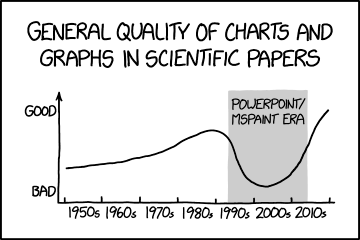
\includegraphics[width=\figwidth]{scientific_paper_graph_quality}
% 	\slcaption{
% 		Developmemt of scientific paper graph quality. A dip in the
% 		quality of scientific graphs is observed from the early 1990s to the early 2010s.
% 		During this time Microsoft Paint and PowerPoint were often used to create graphs in scientific papers.\label{fig:scientific_graph_quality}}
% \end{figure}

% \begin{table}[H]
% 	\begin{tabular}{@{}ll@{}}
% 		\toprule
% 		year & quality \\ \midrule
% 		1985 & good    \\
% 		2000 & bad     \\ \midrule
% 		2015 & better  \\ \bottomrule
% 	\end{tabular}
% 	\caption{
% 		Empirical measurements of scientific graph quality. Data points were collected using
% 		a systematic literature review.\label{tab:scientific_graph_quality}}
% \end{table}
% This references a \figref{fig:scientific_graph_quality} while this references a table \tabref{tab:scientific_graph_quality}.

% A citation looks like this \cite{hadash2018estimate}. To embed a citation in the text flow use textcite,
% \eg \textcite{hadash2018estimate} said you should use a lot of citations.

\section{What do I want to do in this thesis?}


\begin{figure}[H]
	\centering
	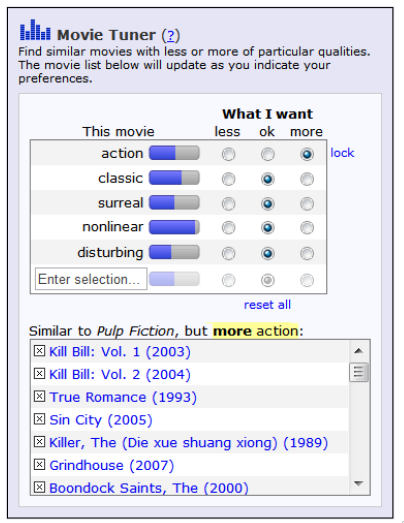
\includegraphics[width=0.7\textwidth]{graphics/stolenfigures/movietuner.png}
	\slcaption{
		The Movie-Tuner Interface from \cite{VISR12}
		\label{fig:movetuner}}
\end{figure}

\subsection{Open Science and Reproducibility}

I think it is absolutely crucial for all branches of science to adhere to the principles of open science and to ensure that all claims that are made in publications are reproducible and testable. This thesis will mostly copy the work of somebody else, but doing so was incredibly tedious, much more so than it would have to be.

Dabei ist mir aufgefallen dass die schon einige DInge machen die ich aus wissenschaftlicher Sicht für ziemlich kritikwürdig halte, zum Beispiel sind die so schwammig in den Formulierungen dass man beim Versuch den Code zu reproduzieren echt viel raten muss, haben geschrieben dass der Code open ist verweisen aber auf ein leeres Repo, haben ihre Daten veröffentlicht aber wenn man damit arbeitet merkt man dass das die selbst definitiv nicht mit dem Datensatz den sie veröffentlicht haben gearbeitet haben könne, sind sehr hart am cherry-picken in ihrer qualitativ  analysis etc etc et

So one main motivation is to reproduce the code for the paper I liked in a way that adheres to the principles of open science, such that others that find it interesting don't have to go through the shit I had to go through.

Principles of open science (TODO: which are: [see thisandthis paper]) are very important to me, so I want to ensure that the claims I am making in this thesis are backed by code that is scalable, reproducible, modular, easily-understood, easily set up and run, well documented, ... . To support this, I will as often as necessary refer to the actual code in this thesis, to allow to understand and reproduce the claims and results, and also highly encourage to critically read everything here and check the respective code (...and let me know if you spot any errors! Just open a Github Issue!)

% TODO: also make the data available somewhere open!


\chapter{Theoretical Background}
% (zuspitzung von generell auf spezifisch, sowohl technisch (conceputalspaces -> was macht das paper konkret), (und bei dem anderen teil was sind educational resources, was sind die schwierigkeiten dabei, warum möchte man überhaupt empfehlen))

\section{Use Case: Educational Resources}
% Anwendungsfall (->e-learning, recommenden von bildungsressourcen, ...) -> nicht-technisch, aber nötig zum verstehen wo passiert das 

\section{Conceptual Spaces}

% \cite{Alshaikh2019} (verbatim!):
% * vector space models that are aimed at representing the entities of a given kind (e.g. movies), to- gether with their associated properties (e.g. scary) and concepts (e.g. thrillers).
% * As such, they are similar in spirit to the vector space models that have been proposed in information retrieval (Deer- wester et al., 1990) and natural language pro- cessing (Turney and Pantel, 2010; Mikolov et al., 2013), but there are also notable differences.
% * First, in the context of conceptual spaces, an explicit dis- tinction is made between the entities from the do- main of discourse, which are represented as vec- tors, and the corresponding properties and con- cepts, which are represented as regions (e.g. poly- topes) or soft regions (e.g. characterized by a Gaussian). 
% * Second, conceptual spaces are organ- ised into a set of facets [domains], each of which captures a different aspect of meaning. For instance, in a conceptual space of movies, we may have facets such as genre, language, geographic location, etc. Each facet is associated with its own vector space, which intuitively captures similarity w.r.t. the corresponding facet. Most of these facet spaces tend to be low-dimensional (e.g. modelling budget only needs a single dimension). This clearly dif- ferentiates them from traditional semantic spaces, which often have hundreds of dimensions






\@input{pandoc_generated_latex/chapter_theobg_section_cs}


\section{Automatic Data-Driven Generation of Conceptual Spaces}

% \cite{Alshaikh2019} geht drauf ein warum man infoGAN und VAEs für bilder als pretty much sowas betrachten kann

%Wie funktioniert die Idee des data-driven generieren 

% Base idea: [Derrac and Schockaert, 2015] proposed an unsupervised method which uses text descriptions of the considered entities to identify se- mantic features that can be characterized as directions. Their core assumption is that words describing semantically mean- ingful features can be identified by learning for each candi- date word w a linear classifier which separates the embed- dings of entities that have w in their description from the oth- ers. The performance of the classifier for w then tells us to what extent w describes a semantically meaningful feature. 
% This method trains for each word w in the vocab- ulary a linear classifier which predicts from the embedding of an entity whether w occurs in its description. The words w1, ..., wn for which this classifier performs sufficiently well are then used as basic features. To assess classifier perfor- mance, Cohen’s Kappa score, which can be seen as a correc- tion of classification accuracy to deal with class imbalance, is used. Each of the basic features w is associated with a cor- responding vector dw (i.e. the normal vector of the separat- ing hyperplane learned by the classifier). These directions are subsequently clustered, which serves to reduce the total num- ber of features.

\section{Types of Reasoning}

\@input{pandoc_generated_latex/chapter_theobg_section_reasoning}

\chapter{Related Work}

% dass das alles vergleichbar mit InfoGAN etc für Bilder ist.. (siehe auch text von \cite{Alshaikh2019})

\@input{pandoc_generated_latex/chapter_related_work}

\chapter{Methods}
%(Algorithmus & Datensatz)

\section{Dataset}

%TODO https://tex.stackexchange.com/questions/526198/table-resize-table-and-automatic-line-breaks
%TODO add back key feature sizes?!
\begin{landscape}
	\begin{table}[]
		\resizebox{\textwidth}{!}{%
			\begin{tabular}{@{}llllll@{}} %l
				\toprule
					\textbf{dataset} &
					\textbf{contents} &
					\textbf{preprocessing} &
					\textbf{size} &
					\textbf{classification classes} &
					\textbf{candidate word threshold}
					% & \textbf{key feature sizes} 
					 \\ \midrule
				\textbf{movies\footnote{\label{origdsets}\url{https://www.cs.cf.ac.uk/semanticspaces/}} \cite{Derrac2015} \cite{Ager2018} \cite{Alshaikh2020} } &
					grouped-by-movie-concatenated reviews for movies &
					\cite{Derrac2015}: removed stop-words\footnote{\label{fnote:stopwordlist}\url{http://snowball.tartarus.org/algorithms/english/stop.txt}}, lower-cased all, removed diacritics and punctuation &
					\specialcell[l]{\cite{Derrac2015}: 15000 movies \\ \cite{Ager2018}/\cite{Alshaikh2020}: 13978 movies } & %Ager2018 says 15.000 - 1022 duplicates, that's the number of Alshaikh2020
					\specialcell[l]{ \tabitem genre (23 classes)\\ \tabitem plot keywords (eg. \textit{suicide, beach}) (100 classes) \\ \tabitem age-rating certificates (6 classes)} & \specialcell[l]{$\geq$ 100 occurences (doq-freq) \\ \textrightarrow around 22k candidates \\ variable-length \textbf{n-grams} considered}
					% & \specialcell[l]{feature vectors: 38649 keys with 0-33k (mostly ~3-6k) unique terms each (in sum 589727 terms) \\ candidate-terms: 22903 (unclustered)\\ clusters: ndims*2 clusters with all in all (for 20d) 9389 values (so 9429 words in $T^{0.1}$)}		
					\\ \midrule
				\textbf{place types\footref{origdsets} \cite{Derrac2015} \cite{Ager2018} \cite{Alshaikh2020} } &
					bag-of-tags from Flickr used to describe places of a certain place-type & 
					None &
					1383 place-types & %both in DESC15 and the follow-up paper
					\specialcell[l]{ \tabitem category from Geonames (7 classes)\\ \tabitem category from Foursquare (9 classes)\\ \tabitem category from OpenCYC (\cite{Derrac2015}: 93 classes, \cite{Ager2018} \cite{Alshaikh2020}: 20 classes) } &
					\specialcell[l]{ $\geq$ 50 occurences (doq-freq) \\ \textrightarrow around 22k candidates \\ (all words from the BoW) \\ \textbf{n-grams}: squashed all words of a tag}
					\\ \midrule
				\textbf{wines\footref{origdsets}\footnote{\url{https://snap.stanford.edu/data/web-CellarTracker.html}} \cite{Derrac2015}} &
					grouped-by-wine-variant concatenated reviews for wines &
					removed stop-words\footnoteref{fnote:stopwordlist}, lower-cased all, removed diacritics and punctuation &
					330 wine-variants &
					\textit{not performed} &
					\specialcell[l] {$\geq$ 50 occurences (doq-freq) \\  \textrightarrow around 6k candidates }
					\\ \midrule
				\textbf{20 newsgroups\footnote{\url{http://qwone.com/~jason/20Newsgroups}} \cite{Ager2018}} &
					posts partitioned (nearly) evenly across 20 different newsgroups &
					\specialcell[l]{ \tabitem Headers, footers and quote metadata removed using scikit-learn \footnote{\url{https://scikit-learn.org/0.19/datasets/twenty_newsgroups.html}} \\ \tabitem removed stopwords (using NLTK's corpus \cite{loper-bird-2002-nltk})\\ \tabitem lowercased text\\ \tabitem candidate terms: all textual and numerical tokens} &
					18446 posts &
					\tabitem newgroup post was submitted to (20 classes) &
					$\geq$ 30 occurences 
					\\ \midrule
				\textbf{imdb sentiment\footnote{\url{http://ai.stanford.edu/~amaas/data/sentiment/} \cite{maas-EtAl:2011:ACL-HLT2011}} \cite{Ager2018}} &
					highly polar movie reviews for binary sentiment classification  &
					\specialcell[l]{ \tabitem removed stopwords (using NLTK's corpus \cite{loper-bird-2002-nltk})\\ \tabitem lowercased text\\ \tabitem candidate terms: all textual and numerical tokens} &
					50000 reviews &
					\tabitem sentiment of the review (2 classes) &
					$\geq$ 50 occurences
					\\ \midrule
				\textbf{Bands \cite{Alshaikh2020}} &
					\specialcell[l]{All Wikipedia pages ($\geq$ 200 words) whose \\ WikiData semantic type is "Band"} &
					\specialcell[l]{ \tabitem removed HTML-tags and references \\ \tabitem \textit{"standard preprocessing strategy"} \cite[137]{Alshaikh2019} \\ \tabitem removed stopwords (using NLTK's corpus \cite{loper-bird-2002-nltk})\\ \tabitem POS-tagging and keeping only nouns and adjectives \\ \tabitem remove words with a rel. doc-freq  $>$ 60\% or abs. doc-freq $<$ 10 } &
					11448 bands & \specialcell[l]{ \tabitem Genres (22 classes) \\ \tabitem Country of origin (6 classes) \\ \tabitem Loc. of formation (4 classes) }  & 
					\specialcell[l]{ 10 $<$ doc-freq $<$ 6869 \\ (all words from the BoW)}\\ \midrule
				\textbf{Organisations\footnote{\label{fnote:for_alshaikh2019} Originally created in and for \cite{Alshaikh2019}} \cite{Alshaikh2020}} &
					\specialcell[l]{All Wikipedia pages ($\geq$ 200 words) whose \\ WikiData semantic type is "Organisation"} &
					\specialcell[l]{ \tabitem removed HTML-tags and references \\ \tabitem \textit{"standard preprocessing strategy"} \cite[137]{Alshaikh2019} \\ \tabitem removed stopwords (using NLTK's corpus \cite{loper-bird-2002-nltk})\\ \tabitem POS-tagging and keeping only nouns and adjectives \\ \tabitem remove words with a rel. doc-freq  $>$ 60\% or abs. doc-freq $<$ 10 } &
					11800 organisations &
					\specialcell[l]{ \tabitem Country (4 classes)\\ \tabitem Headquarter Loc. (2 classes)} &
					\specialcell[l]{ 10 $<$ doc-freq $<$ 7080 \\ (all words from the BoW)} \\ \midrule
				\textbf{Buildings\footnoteref{fnote:for_alshaikh2019} \cite{Alshaikh2020}} &
					\specialcell[l]{All Wikipedia pages ($\geq$ 200 words) whose \\ WikiData semantic type is "Building"} &
					\specialcell[l]{ \tabitem removed HTML-tags and references \\ \tabitem \textit{"standard preprocessing strategy"} \cite[137]{Alshaikh2019} \\ \tabitem removed stopwords (using NLTK's corpus \cite{loper-bird-2002-nltk})\\ \tabitem POS-tagging and keeping only nouns and adjectives \\ \tabitem remove words with a rel. doc-freq  $>$ 60\% or abs. doc-freq $<$ 10 } &
					3721 buildings &
					\specialcell[l]{ \tabitem Country (2 classes)\\ \tabitem Administrative loc. (2 classes)} &
					\specialcell[l]{10 $<$ doc-freq $<$ 2233 \\ (all words from the BoW) }\\ \midrule \midrule
				\textbf{Siddata-Courses} &
					TODO &
					&
					&
					\tabitem Faculty (10 classes) 
					\\ \midrule 
				\textbf{100K Coursera reviews}\footnote{\url{https://www.kaggle.com/septa97/100k-courseras-course-reviews-dataset}} &
					TODO &
					&
					&
					\specialcell[l]{ \tabitem Rating (5 classes) \\ \textit{\tabitem Major, Category, Offered-By,... (tbd)} }
					\\ 
			\end{tabular}
			\caption{All datasets. Extends similar table in \cite{Alshaikh2020}}
			\label{tab:all_datasets}
		}
	\end{table}
	% TODO was ist mit n>1-grams? Movies used them, placetypes used tags so it kinda has them... and stuff liek buildings/organizations?
\end{landscape}	

% Empirie, auch specifics über den Datensatz

%To write:
% * where does the data come from
% * what size is the data, what is the distribution, ...
% * Preliminary analysis (if I delete all that are shorter than X, it are |Y|..)
% * Does it cluster and look nice?
% * Verteilung der Sprachen
% * Preprocessing in kurzem Fließtext beschreiben - "After throwing out all descriptions shorter than xyz chars, 2323 courses where left. 223 of these were ..."
% * That the type of dataset differs from DESC15 and followups - mainly used movie-dataset consists of concatenated reviews (which means relevant words occur more often!) 
%     (TODO: look/think was die anderen auszeichnet - bei dem placetypedataset ists ja gar kein fließtext sondern direkt ein bag-of-tags)
% Dass mein Datensatz kleiin ist! Bei keinem sonderlichen min-word-per-desc threshold hab ich halt 7588 samples, bei 50 schon nur noch 4123, das ist wirklich little
% Dass auch die Descriptions echt kurz sind! Ich hab rund 8k samples, um das selbe samples-to-threshold verhältnis zu haben wie DESC15 wäre rechnerisch ein wert von 2 bis 25 sinnvoll (wobei man beachten muss das 2 schon richtig kacke ist weil dann die SVM 2 vs 8000 klassifizieren muss and that will never work -> 25 ist minimum), ABER wenn ich dann 25 nehme hab ich nur 2.4k candidates statt the 22k DESC15 aimed at, which also sucks!! --> CONCLUSION: Datensatz scheint zu klein.

The main goal of this thesis was to create a conceptual space of courses, automatically generated by course descriptions.


For that, a dataset of courses and their descriptions was obtained as export from the Stud.IP system as used at the universities of Osnabrück, Hannover and Bremen.
%TODO wait, woher kam der datensatz überhaupt? Tobias hat mir den geschickt, aber kam er zustande im Rahmen von Siddata?

The dataset comes from Johannes' Repo at \url{https://git.siddata.de/jschrumpf/study_behavior_analysis} (requires authentification over UOS!)

\begin{figure}[H]
	\centering
	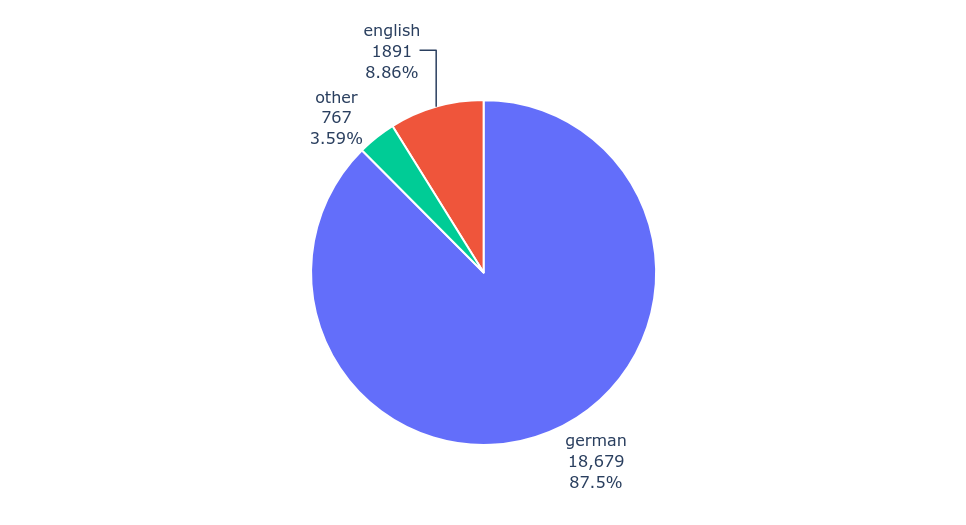
\includegraphics[width=\figwidth]{graphics/figures/courses_language_distribution.png}
	\slcaption{
		\label{fig:courses_language_distribution}
		Distribution of languages of course descriptions.
		%TODO figure if this is the correct amount of preprocessing/throwout to have done
		Of the 21337 courses left after preprocessing, 18,679 were in german language according to the \textit{langdetect} python-package\footnote{\url{https://pypi.org/project/langdetect/}, which is a direct port of a java library\ which claims to have 99.8\% accuracy on longer texts\cite{nakatani2010langdetect}}.
		}
\end{figure}

To see if it is possible to extract any kind of structured data from the unstructured course descriptions, a Neural Network classifier was trained on the dataset, classifying courses to the faculty they run under. 
The faculty is easily obtainable from the dataset, as the first one or two digits of the course ID correspond to it. The distribution of the faculties is depicted in figure \ref{fig:faculty_plot}.

\begin{figure}[H]
	\centering
	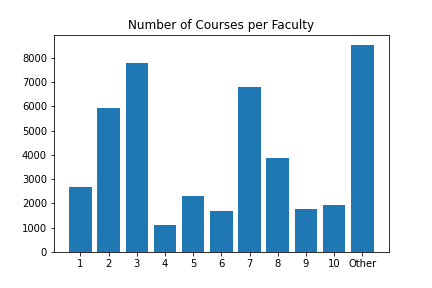
\includegraphics[width=\figwidth]{graphics/figures/faculty_plot.png}
	\slcaption{
		\label{fig:faculty_plot}
		Distribution of faculties in the courses
		}
\end{figure}

The purpose of the Neural Network classifier is to check if it is anyhow possible to extract meaningful information from the descriptions: If it is possible to train a classifier on the data that can reasonably predict a qualitative feature, there is enough structure in the data such that the algorithm I'm about to produce can work.
Also, we have a lower bound for useful data: we can just throw away data that cannot be classified!
%TODO: train a second classifier on something else and throw away data that gets classified by neither and inspect it

(-> 91\% test accuracy)

\subsection{Other Datasets}

%TODO: write IN THE ALGORITHM & ARCHITECTURE SECTIONS that I of course tried the placetypes-dataset as sanity-check to find errors - for that dataset, stuff like the good-candidates is known so as long as I don't reach their performances for that dataset I know my code is the problem, but as soon as I reach their performance I can savely say that the actual algorithm is correct and if it's still bad on the siddata dataset it's just not applicable to this kind of data

Also tried the Plactypes-Dataset used by all main-paper-authors. When doing so I noticed that there are definitely duplicates (which are consistently recognized as closest-terms in embedding):
  abandoned rail road and abandoned railroad
  boat yard and boatyard
  coral reef and reef
  court house and courthouse
  grass land and grassland
  sheep fold and sheepfold
  skate park and skatepark
  steak house and steakhouse
  water fall and waterfall
  wind mill and windmill

Next to that, the embedding however also sees very similar ones as very similar, which is a nice sanity-check, eg.

  abandoned farm and abandoned home
  airfield and airport
  airport and airport terminal
  ancient site and archaeological site
  arch and arch bridge
  art gallery and art museum
  coffee house and coffee shop
  aircraft cabin and airplane cabin
  apartment and apartment building
  bank and bank building
  field hockey field and hockey field


Also tried a dataset of 100.000 coursera course reviews from \url{https://www.kaggle.com/septa97/100k-courseras-course-reviews-dataset}. Why? Because it's also eduactional resources, but as it's reviews it seems closer to the movies dataset
See \url{https://www.kaggle.com/roshansharma/coursera-course-reviews} for exploratory analysis of the dataset (there he also has another dataset he writes about, but you cannot merge them unfortunately, so besides course name the only possible task is the rating)
%TODO: I could try to merge it with this one https://www.kaggle.com/siddharthm1698/coursera-course-dataset or another one (see https://www.kaggle.com/mihirs16/coursera-course-data which links names to links, https://www.kaggle.com/search?q=coursera+in%3Adatasets for other places)

Also, there's the Large Movie Review Dataset\footnote{\url{http://ai.stanford.edu/~amaas/data/sentiment/}, \url{https://scikit-learn.org/0.19/datasets/twenty_newsgroups.html}}, also used by \cite{Ager2018}.


\section{Required Algorithms and Techniques}

The Paper uses the following PPMI definition:\\ 

\noindent $e \in E$ is an entity, $D_e$ a document (bag of words) where that entity occurs.\\
We want to quantify for each term occuring in the corpus $\{D_e | e \in E\}$ how strongly it is associated with $e$.\\
$c(e,t)$ is the number of times term $t$ occurs in document $D_e$. \\
The weight $ppmi(e,t)$ for term $t$ in the vector representing $e$ is then:
\begin{align*}
ppmi(e,t) &= max\left(0, log\left( \frac{p_{et}}{p_{e*}*p_{*t}} \right) \right) \\
          &= max\left(0, pmi(e,t) \right) \\
 pmi(e,t) &= log\left( \frac{p_{et}}{p_{e*}*p_{*t}} \right) \\          
   p_{et} &= \frac{c(e,t)}{\sum_{e'}\sum_{t'} c(e',t')} \\
   p_{e*} &= \sum_{t'}p_{et'} \\
   p_{*t} &= \sum_{e'}p_{e't} \\
\end{align*}

\noindent log of the probability of the $e$-$t$-combination (count of this vs count of all), normalized by the probability of this $e$ with any $t$ times this $t$ with any $e$.\\
To quote the paper: "PPMI will favor terms which are frequently associated with the entity $e$ while being relatively infrequent in the corpus overall"

\vspace{30px}

I found this definition:
\begin{align*}
ppmi(X,i,j) &= max(0, pmi(X,i,j)) \\
pmi(X,i,j)  &= log\left( \frac{X_{ij}}{expected(X,i,j)} \right) \\
            &= log\left( \frac{P(X_{ij})}{P(X_{i*}) * P(X_{*j})} \right)
\end{align*}


\@input{pandoc_generated_latex/chapter_methods_section_required_algorithms}

\section{Architecture}
%Doing this section before Algorithm-section such that I can reference how plots are created or general code examples with the real thing, including how what you're seeing was generated and can be reproduced

%TODO: Also in this chapter:
% * Source-code is ofc open, available under github under this link, it is referred to the signed commit xyz
% * Reference Snakemake-Paper (and at least look a the abstract of that, they also talk about that in science you need reproducible, adaptable and transparency including definitions of what that means!)
\cite{Molder2021a}
% 		* good way to bash the original paper who either didn't publish their sourcecode or link a github-repo in their paper that is fucking empty, or did at least opensource their code but have just one fucking file in there that expects >40 unnamed command-line-args


\@input{pandoc_generated_latex/chapter_methods_section_architecture}



\section{Algorithm}

The algorithm that is implemented in the scope of the thesis is in principle the one from \cite{Derrac2015}, but includes some changes from \cite{Ager2018} \cite{Alshaikh2020}. All of these share Prof. Steven Schockaert as last author, which makes me assume a) the latter ones are legit improvements upon the first, b) at least to a certain degree they can share code and data, c) afaik there are no other imlementations of this anywhere
% General idea of the algorithm: Alshaikh2020: "Their core assumption is that words describing semantically meaningful features can be identified by learning for each candidate word w a linear classifier which separates the embeddings of entities that have w in their description from the others. The performance of the classifier for w then tells us to what extent w describes a semantically meaningful feature" (TODO: my concise formulation)
% TODO: despite my citation style, write the names of the three main papers at least once

Das haupt-ziel der algorithmen ist es, am ende die entities "feature-based" darstellen zu können, also als high-dim-vector mit floats per human-interpretable dimension. Alshaikh2020 hat dafür wegen den subfeatures noch kleine specials

Important features:
\begin{itemize}
	\item Unsupervised (in constrast to \cite{VISR12})
\end{itemize}

%TODO: maybe describe shortly what the improvements from  \cite{Ager2018} and \cite{Alshaikh2020} were? 
% Alshaikh2020: 
% * "When representing a particular entity in a conceptual space, we need to specify which domains it belongs to, and for each of these domains we need to provide a corresponding vector." 
% * then they show their example of something that is not seperable with a hyperplane unless we specify subdomains, maybe just steal their plot that explains their one contribution to 99%
% * The "Disentangled" from their title means "feature-based"

The core idea of the algorithm is to (unsupervised, data-driven) find a a set of features which can be modelled as directions for a vector-space representation of the respetive entities. For that, the steps are:
\begin{enumerate}
	\item preprocess the descriptions using default techniques and create a bag-of-words representation for the texts
	\item extract candidate features from these texts (easist variant is to just consider each sufficiently frequent word as candidate)
	\item create an fixed-dimensional embedding for the texts (optimally a metric space, optimally based on their dissimilarity)
	\item for each candidate term, train a linear classifier to seperate the vector representationgs of the entities that contain the term vs those that don't
	\item if some metric for this classifier is sufficiently high, assume that the candidate term captures a salient feature - it's direction is then characterized by the normal vector for that hyperplane (for an intuition see \ref{fig:3d_hyperplane_ortho})
	\item Cluster the candidates and calculate the direction of the cluster from the directions of it's contents
\end{enumerate}

\begin{figure}
	\begin{center}
	  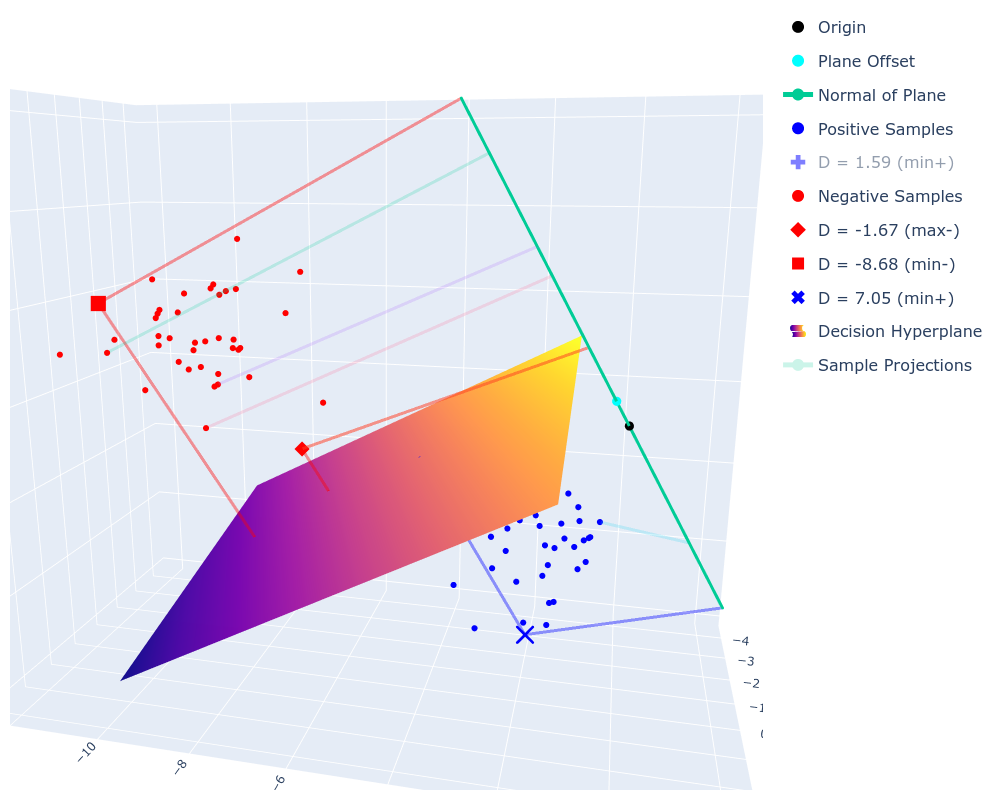
\includegraphics[width=0.9\textwidth]{3dplot_hyperplane_and_orthogonal}
	  \caption[Visual representation of the Hyperplane of an SVM splitting a dataset]{ \label{fig:3d_hyperplane_ortho} Visual representation of the Hyperplane of a Support-Vector-Machine splitting a dataset, as well as it's orthogonal and the orthogonal projection of a set of samples onto the plane. For an interactive version of this plot, visit  {\small \url{https://nbviewer.org/github/cstenkamp/derive_conceptualspaces/blob/main/notebooks/text_referenced_plots/hyperplane_orthogonal_3d.ipynb?flush_cache}}}
	\end{center}
\end{figure}

\begin{figure}[htp]
	\begin{center}
	  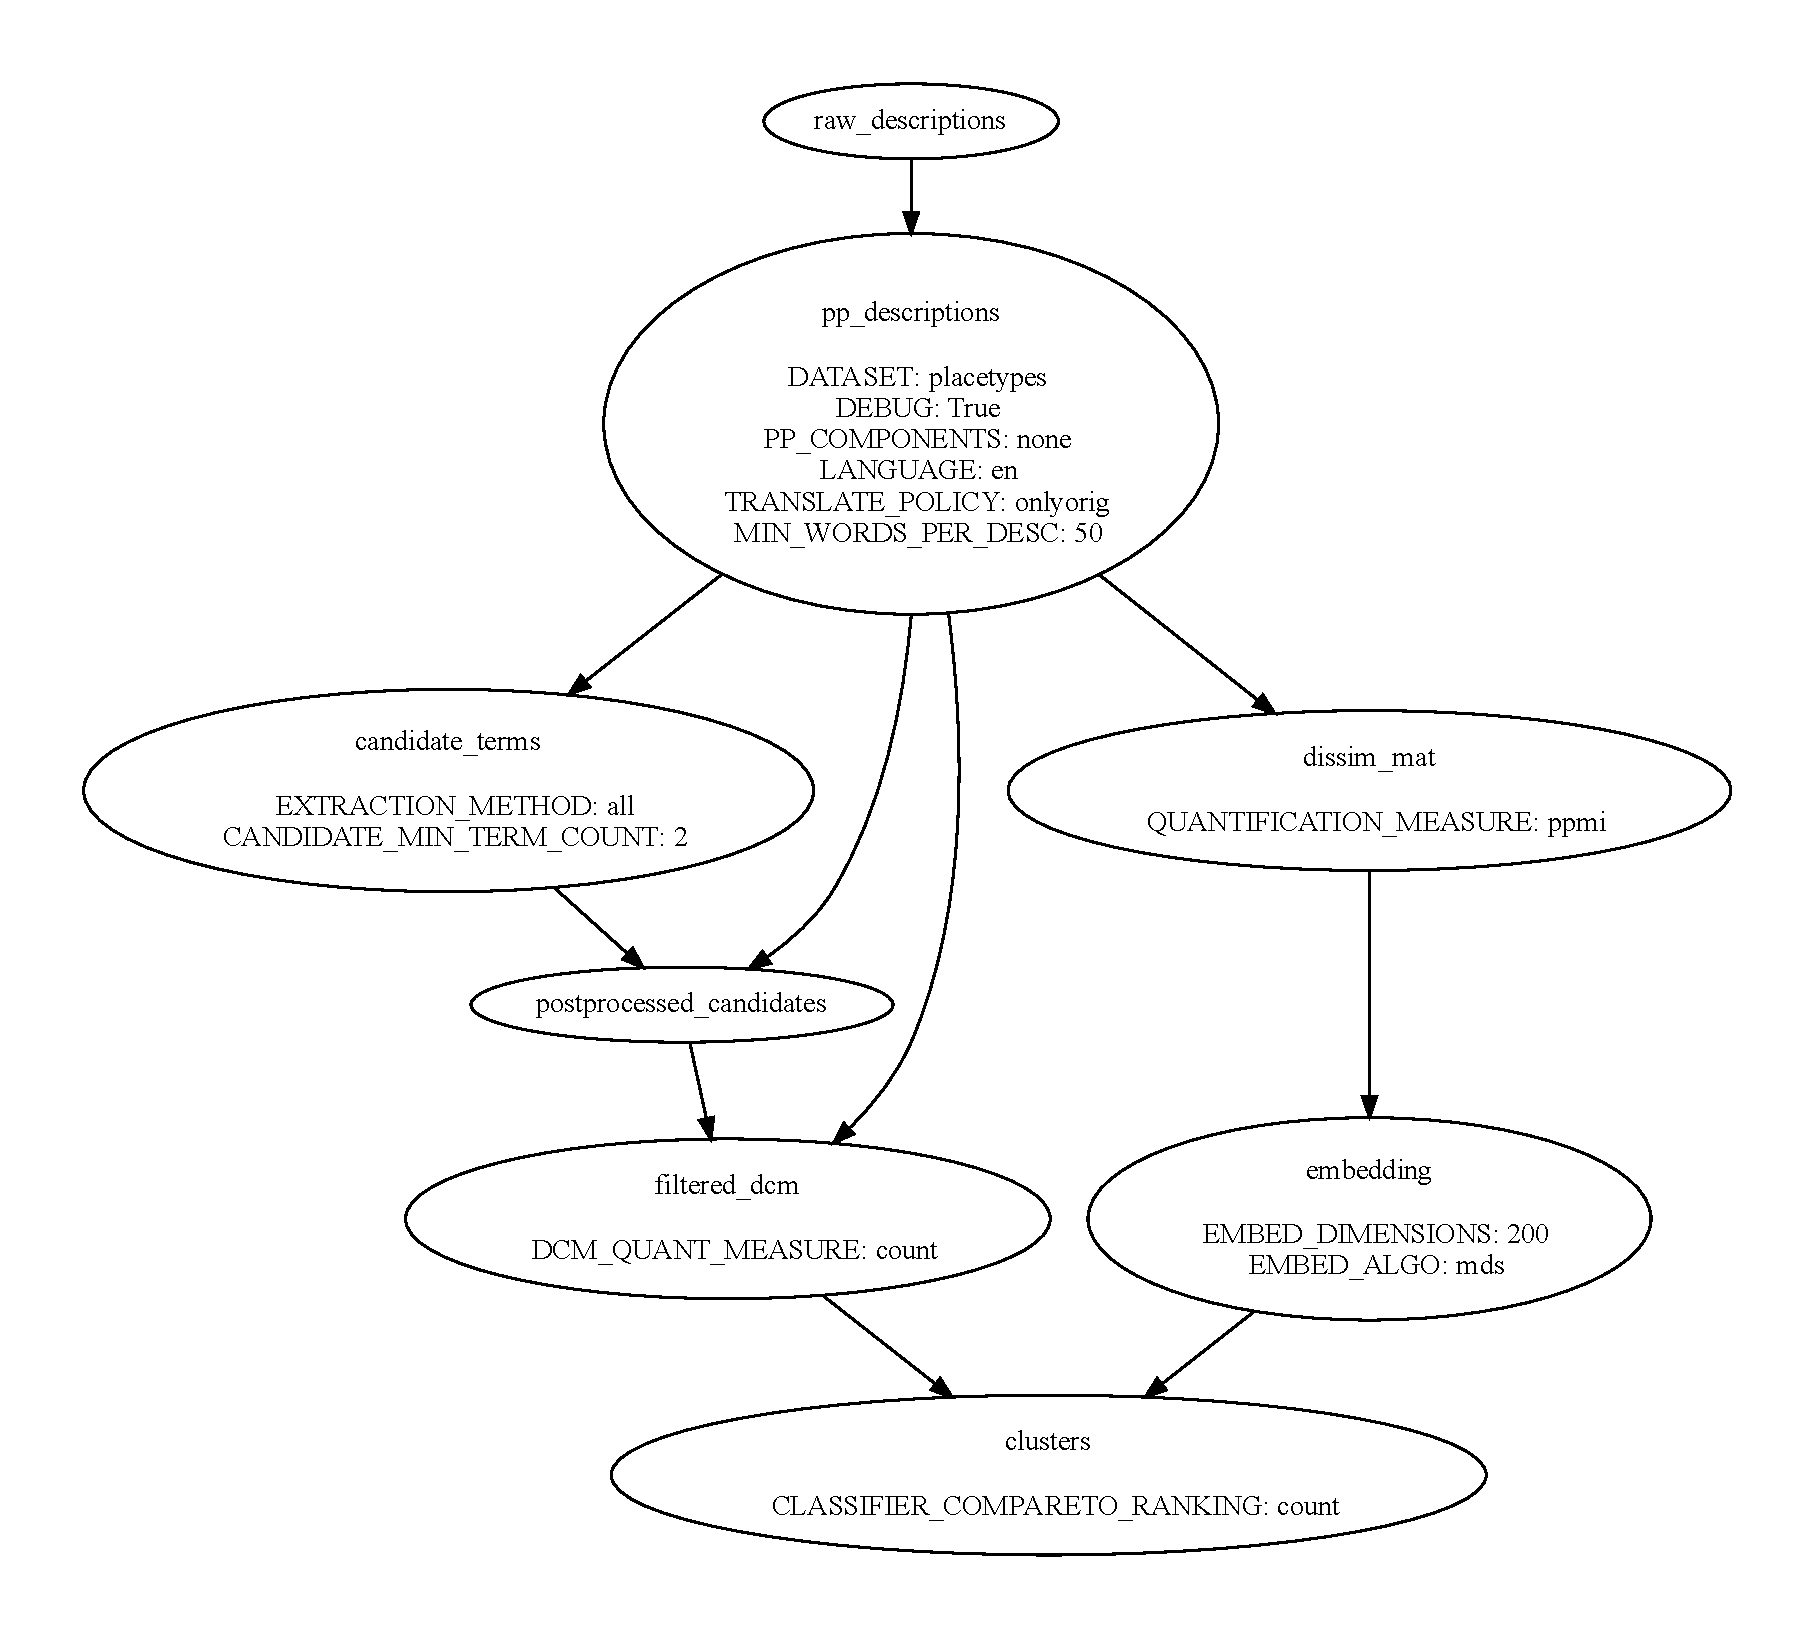
\includegraphics[width=0.9\textwidth]{dependency_graph_2022-02-14_11-36-45}
	  \caption[Dependency-Graph of the Algorithm]{(automatically generated) dependency-graph, displaying the individual steps of the algorithm as well as their dependencies and where selected important parameters are first used.}
	  \label{fig:depdendency_graph}
	\end{center}
\end{figure}

\@input{pandoc_generated_latex/section_algorithm}




\begin{landscape}
	\begin{table}[]
		%Preprocessing siehe other table
		\resizebox{\textwidth}{!}{%
			\begin{tabular}{llll}
			& \cite{Derrac2015} & \cite{Ager2018} & \cite{Alshaikh2020} \\
			\textbf{Step 1: Generate Vector Spaces from Descriptions} & 
			\specialcell[l]{MDS trained with the angular differences $\frac{2}{\pi}* arccos\left(\frac{\vec{v}_{e_i}*\vec{v}_{e_j}}{\norm{\vec{v}_{e_i}}*\norm{\vec{v}_{e_j}}}\right)$ \\
			between the PPMI weighted BoW Vectors (all terms) \\
			Spaces of dim 20, 50, 100 and 200 \\
			Previous Experiments also considered SVD and Isomap} &
			\specialcell[l]{ \tabitem like \cite{Derrac2015} \\ \tabitem PCA from PPMI weighted BoW vectors \\ \tabitem Doc2Vec \\ \tabitem thresholded\footnote{Only words that occur more than 2 times (15 for movies-dataset)}, averaged pre-trained GloVe word embeddings \\ \tabitem thresholded, ppmi-weighted-averaged pre-trained GloVe word embeddings \\
			Number of dimensions one of (50, 100, 200)} &
			\specialcell[l]{ \tabitem Document Embeddings } \\ \midrule
			\textbf{Step 2: Generate Candidate Words for Features} & 
			\specialcell[l]{ All sufficiently frequent\footnote{For the placetypes-dataset: all tags that co-occur with at least 50 place types} adjectives, nouns, adjective phrases and noun phrases \\
			(using POS-Tagger and Chunker from openNLP) } &  
			All sufficiently frequent words\footnote{For the thresholds, see table \ref{tab:all_datasets}} (use PPMI in a later step so possibly PPMI?!) &
			\\ \midrule
			\textbf{Step 3: Filter Candidate Words} &                   
			\specialcell[l]{ linear SVM for all candidates (pos samples: $\forall e: c \in e$) with pos/neg-count-ratio as instance cost \\
			Only take candidates where the correlation according to Cohen's Kappa between the ranking induced by the SVM's hyperplane and count(t, e) is $\geq \lambda$ (0.5/0.1)\\
			also tried Spearman's and Kendall's correlation coeffcients }&
			\specialcell[l]{ Performance of the weighted LogRegClassifier compared to the ranking induced by the PPMI, as measured by \\ \tabitem Cohen's Kappa \\ \tabitem Accuracy \\ \tabitem Normalized Discounted Cumulative Gain (NDCG) } 
			& "we used logistic regression classifiers instead of SVMs, which we found to perform similarly but were faster to train."
			\\ \midrule
			\textbf{Step 4: Merge Candidate Word Feature Directions} &   
			\specialcell[l]{ According to \cite{Alshaikh2020} "a variant of \textit{k}-means" \\ Cluster centers: Select Term with highest $\kappa$, then i=2*ndims times select the term from $T^{0.5}$ minimizing $max_{j<i}cos(\vec[m]{v_{t_j}},\vec[m]{v_t})$ \\ 
			Others: assign all terms from $T^{0.1}$ to the closest cluster and define $\vec[m]{v^*_i} = \frac{1}{|C_i|} \sum_{t\in C_i} \vec[m]{v_t}$ as cluster direction (average direction of cluster's elements)} &
			\specialcell[l]{Weighted logistic regression to find candidate directions \\ 
			Input-ndims for clustering algorithm one of (500, 1000, 2000) \\
			Number of clusters one of (ndims, 2*ndims) \\
			Centroid of the cluster computed as $v_{C_j} = \frac{1}{|C_j|}\sum_{w_l \in C_j} v_l$, provided vectors all normalized} & \specialcell[l]{  \textbullet\, \textbf{sub, ortho, primary}:   
			Affinity propagation instead of \textit{k}-means (no need to specify the ndims, helps with the issue that there are some non-informative clusters in \cite{Derrac2015}'s algorithm) \\ ~~ n-dims for this not directly configurable, only over preference parameter relative to median $\mu$, tried for (0.7$\mu$, 0.9$\mu$, $\mu$, 1.1$\mu$, 1.3$\mu$) \\  \textbullet\, \textbf{AHC}: Agglomerative Hierachical Clustering to cluster word directions with distance cut-offs  \\  \textbullet\, also tried Hierachical LDA \\ Cluster direction (both AHC and Affinity Propagation): normal vector of the hyperplane of a linear classifier separating entities whose description contains at least one of the words from the cluster from the others  } %TODO find a short-term notation for "entities whose description contains at least one of the words from XYZ" ("for a Cluster C, we write pos_C and neg_C for the set of positively and negatively classified entities")
			\\  \midrule
			\textbf{Step 5: Post-Processing} &                   
			None &                 
			TODO describe fine-tuning! & \specialcell[l]{
			Perform steps 1-4 a second time (only for positively classified entities), such that there are primary features (domains) and sub-features \\ representation kept flat (values for the sub-features is same dot-product as for domains) \\ \textbullet\, \textbf{sub}: sub-features extracted equal to first-order-features \\ \textbullet\, \textbf{ortho}: sub-feature directions orthogonal to corresponding primary feature direction (enforce complementary information) \\ ~~ by computing orthogonal decomposition of feature w.r.t. its domain (pg. 4, equation 1) \\ \textbullet\, also tried to combine mother-domain with sub-feature, but that performed poorly \\ \textbullet\, \textbf{primary}: model with only primary features}
			\end{tabular}
		}
		\caption{Compared algorithms from \cite{Derrac2015} \cite{Ager2018} \cite{Alshaikh2020}}
		\label{tab:compared_algos}
	\end{table}
\end{landscape}

% Alshaikh2020 say: "It may seem counter-intuitive to use binary classifiers to learn representations of ordinal features. However, the occurrence or non- occurrence of a word in the description is binary, and this is the most important available signal. We experimented with statistics such as pointwise mutual information, which did not lead to better results." -> does that mean DCM_QUANT_MEASURE or QUANTIFICATION_MEASURE or both? and also does that mean they use binary or count as this measure?

% Alshaikh2020 use: sub, ortho, primary, random (coordinates uniformly random), 


\subsection{Preprocessing}

There are issues with using stop-word lists, see \cite{nothman-etal-2018-stop} ( SkLearn references this paper why their own/stopwordslists in general suck)


%Was für Schritte hat der Algo 

%TODO something along the lines of "Da, based on [source die die accuracy von dem gtranslate algorithm mit denen von menschen vergleicht], a gtranslate translation is as good as the average lecturer, it is assumed that translating the texts to english before using an english model can lead to better results


\subsection{Extracting Candidate Terms}
\label{sec:extract_candidates}

* KeyBERT

%TODO theoretisch ist es auch möglich bspw nen network mit attention auf gewisse dinge wie fachbereich und anderes zu trainieren und dann rauszusuchen was die wichtigen ausschlaggebenden dinge für das Netzwerk waren

%TODO extract using TF/IDF as well

%TODO a source: https://github.com/MaartenGr/KeyBERT#citation

* After you figure out which candidate term appears in which texts, figure out which other terms are frequent in these texts while infrequent in texts of the other class and then add these to the candidate-term-set (other way may even be to classify the texts according to if the candidateterm appears in them, and then take the misclassified one also as positive samples)

\begin{figure}[H]
	\centering
	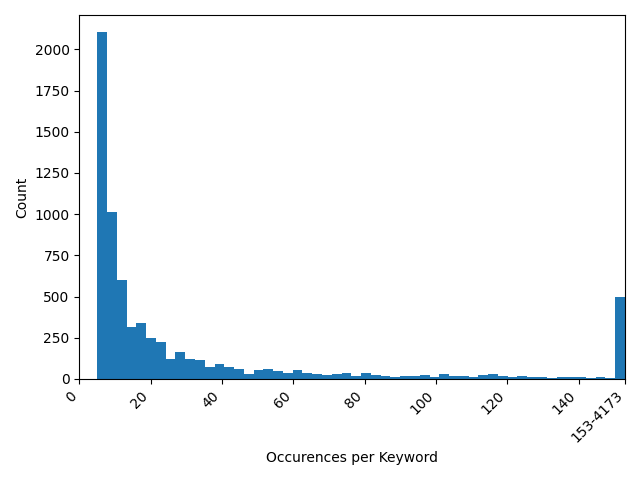
\includegraphics[width=\figwidth]{graphics/figures/keyphrases_histogram.png}
	%plot created with scripts/create_siddata_dataset.py filter-keyphrases /home/chris/Documents/UNI_neu/Masterarbeit/DATA_CLONE --verbose
	\caption[Occurences in all Documents per Keyphrase]{
		\label{fig:keyphrases_histogram}
		Occurences in all Documents per Keyphrase (for all keyphrases that occur $\geq$ 5 times, cut off at the 93th percentile).
		7007 of 45295 terms occur at least 5 times.
		Most frequent phrases: seminar (4173), course (3722), students (2923), it (2671), language (2071), work (1980), event (1842), research (1731), lecture (1723), law (1719).
		}
\end{figure}


\subsection{Calculating the distance to the SVMs Separatrix}
\label{sec:calculate_distance}

%TODO: before this, explain 
% * extraction of the candidate term set
% * how vectors are made from texts
In order to tell how much a text is prototypical of a category, all texts are split depending on whether they contain words of a set as described in \ref{sec:extract_candidates}, before a linear Support Vector Machine Classifier is trained on the vector-representation of all of the texts, splitting them into two classes: those that contain one of the candidate terms and those that do not. Due to the linear kernel, the SVM finds a hyperplane (\textit{separatrix}) that splits the positive from the negative samples in a way that maximizes the distance between the respective classmembers and the separatrix, using samples close to the margin as \textit{support vectors}. %TODO: what if the data is not linearly seperable?

Following the SVMs logic, one could argue that the further away a sample is from this separatrix, the more prototypical it is of its class. Thus, the distance of a sample to its \textit{orthogonal projection onto the hyperplane} %TODO explain orthogonal projection
may serve as metric for how prototypical a sample is for the respective category. 

Translated into terms relevant to the aim of this thesis, the classes may be those educational resources whose description contains the word "\textit{hard}" as one class vs. those that do not as the other class. Now according to [TODO], one may use the distance of the sample towards the separatrix as a measure of how hard a class is: For all positive samples, a longer distance means a harder class, for all negative samples a longer distance means an easier one, whereas those samples close to the separatrix can be considered average.

\subsubsection*{How to calculate the distance}

%TODO mention that I'm in a cartesian coordinate system
%TODO mention that I'm thinking in euclidian coordinates, see https://en.wikipedia.org/wiki/Plane_(geometry)
\noindent In the following paragraphs, I will visualize how to calculate the orthogonal distance from a sample to the hyperplane exemplary for the case of three-dimensional text-vectors.

Generally, the separatrix splitting positive from negative samples for an $n$-dimensional space $\mathds{R}^n$ is an $n-1$-dimensional subspace (called \textit{hyperplane}), which in the case of $\mathds{R}^3$ corresponds to a plane. 
%https://en.wikipedia.org/wiki/Plane_(geometry)#Representation

The general form of the equation of a plane is given as the following linear equation, where parameters $a, b, c$ and $d$ encode the position of the plane:

\begin{equation}
	\label{eq:general_plane}
	ax + by + cz = d
	%TODO source? mein Tafelwerk? :D
\end{equation}

This reads as "All points $(x,y,z)$ for which \ref{eq:general_plane} holds are on the plane". 

In this representation of the plane, the vector $(a,b,c)$ encodes a normal vector orthogonal to this plane, whereas $d$ serves as intercept, encoding the intersection of plane and normal. (specifically: the perpendicular distance you would need to translate the plane along its normal to have the plane pass through the origin) In higher dimensions, the formula for the hyperplane would become $a_1x_1+a_2x_2+a_3x_3+...+a_nx_n = b$, which means that encoding the hyperplane for a space $\mathds{R}^n$ requires $n+1$ parameters.
% one rough quote in this paragraph from https://stackoverflow.com/a/17661431

%TODO explain that it's not even harder in higher-dimensional spaces
%TODO explain that nicely, in python the separatrix is perfectly specified using the normal and the intercept, so we have everything we need 
%TODO die handschriftlichen notizen aus den beiden notebooks einbauen
%TODO die plots aus dem notebook einbauen

% The distance from any point of this $\mathds{R}^n$ to the hyperplane is then calculated as the length of the vector that is the \textit{orthogonal projection} from that point onto the hyperplane. The orthogonal projection from one vector onto another can be calculated as 

% \begin{equation}
% 	\label{eq:orthogonal_projection}
% 	\hat{\vec{a}} = \frac{\vec{a}\cdot\vec{b}}{\vec{b}\cdot\vec{b}}\cdot\vec{b}
% 	%TODO source https://en.wikipedia.org/wiki/Vector_projection
% \end{equation}

% ...as we however have a plane we want to project to, not a vector, what I wrote here is rather useless, isn't it?


The distance from any point of this $\mathds{R}^n$ to the hyperplane can then be calculated as 
% As... * dist(point, point_projected_onplane)     						 (`project[1,3]_pre`)
%       * abs(trafo(point)[0])     										 (`protoypicality_pre`)
%       * np.dot(plane.normal, point) + plane.d							 (`project2_pre')
% ...normiert sind die alle gleich, aber for some reason differn die um nen multiplicator..?!
% And the projections...:
%       * back_trafo([0, trafo(point)[1], trafo(point)[2]]
% 		* plane.project(point): k = (ax+by+cz+d)/(a²+b²+c²); result = [x-ka, y-kb, z-kc]
%       * point - distance * plane.normal  (...aber nur mit protoypicality_pre als distance! )
% 		...note that second and third are basically equal - both calculate "how much do I need to go into the direction of the orthogonal" and then do so  (point - distance * normal). The difference is that in plane.project the distance is divided by (a²+b²+c²). Originally sagt der typ von SO (https://stackoverflow.com/a/17661431) die distance ist einfach n*p-d, dann fehlt nur der normierungsterm. 
% TODO: figure out the explanation of the difference from this to the result of using forward and backward??
% See get_svm_decisionboundary.ipynb, den kram zwischen `#deleteme from here', commit d46a8300dae81adee


\subsection{Clustering the extracted candidates}

An analysis of \cite{Carmel2009} showed that a statistical method to extract features from clustered text corpora identified the labels of human annotators as one of the top five most important terms in only 15\% of cases, implying ``that human labels are not necessarily significant from a statistical perspective" \cite[139]{Carmel2009}
%TODO: die eigentliche Methode (JSD) mehr erklären!!
%(the JSD method for feature selection identifies human labels as “significant” (appearing in the top five most important terms) for only 15% of the categories. This result implies that human labels are not necessarily significant from a statistical perspective.z)


\chapter{Results}


\begin{table}
	\resizebox{\textwidth}{!}{%
	\begin{tabular}{lllllrrrrrrrrr}
	\toprule
	 &  &  &  &  & \rotatebox{45}{\textbf{k_r2r_d}} & \rotatebox{45}{\textbf{k_r2r_min}} & \rotatebox{45}{\textbf{k_dig}} & \rotatebox{45}{\textbf{k_c2r+}} & \rotatebox{45}{\textbf{k_r2r+_d}} & \rotatebox{45}{\textbf{k_r2r+_min}} & \rotatebox{45}{\textbf{k_r2r+_max}} & \rotatebox{45}{\textbf{k_dig+_2}} & \rotatebox{45}{\textbf{mean}} \\
	\rotatebox{45}{\textbf{pp_components}} & \rotatebox{45}{\textbf{quantification_measure}} & \rotatebox{45}{\textbf{embed_dimensions}} & \rotatebox{45}{\textbf{dcm_quant_measure}} & \rotatebox{45}{\textbf{kappa_weights}} &  &  &  &  &  &  &  &  &  \\
	\midrule
	\multirow[t]{5}{*}{\textbf{mfauhcsd2}} & \multirow[t]{5}{*}{\textbf{count}} & \multirow[t]{5}{*}{\textbf{3}} & \multirow[t]{2}{*}{\textbf{count}} & \textbf{linear} & 0 & 0 & 0 & 0 & 0 & 2 & 0 & 0 & 0 \\
	 &  &  &  & \textbf{quadratic} & 0 & {\cellcolor{lightgreen}} 1 & 0 & 0 & 0 & 28 & 13 & 0 & 5 \\
	\cline{4-5}
	 &  &  & \multirow[t]{2}{*}{\textbf{ppmi}} & \textbf{linear} & 0 & 0 & 0 & - & 9 & 30 & 74 & 7 & 17 \\
	 &  &  &  & \textbf{quadratic} & 0 & {\cellcolor{lightgreen}} 1 & 0 & - & {\cellcolor{lightgreen}} 145 & {\cellcolor{lightgreen}} 370 & {\cellcolor{lightgreen}} 510 & {\cellcolor{lightgreen}} 191 & {\cellcolor{lightgreen}} 174 \\
	\cline{4-5}
	 &  &  & \textbf{tfidf} & \textbf{linear} & 0 & 0 & 0 & - & 5 & 18 & 24 & 2 & 7 \\
	\bottomrule
	\end{tabular}
	}
\end{table}
	
	
	
	
	
	
	
	
	
	


\section{Evaluation} %TODO what is this for a title? it sucks


* This is clustering and looking if it corresponds to human judgement, which unfortunately doesn't allow for a simple accuracy and be done with it.
* So, the papers that did this come up with a few things
* [TODO: the shallow decisiontrees of one of the followups]
* DESC15 "evaluate the practical usefulness of the considered semantic relations" by checking "their use in commonsense reasoning based classifiers", like interpolation and a fortiori inference (chap 5)


* DESC15 tests like this: Section 6.1: Evaluate whether the derived relations are sufficiently accurate for classification, and 6.2 is then comparison with crowdsourcing experiments (more subjective aspects, the question “are the relations useful explanations?”)



\section{Qualitative Analysis}

Qualitative Analysis in this case means "looking at stuff". Such a qualitative analysis is always to be taken with a grain of salt, because it is very prone to cherry-picking (both on purpose and not on purpose, the stuff you're looking at just doesn't need to be representative!). However it does help a lot and provides a lot of insights (and often helped me in the debugging process).
What can you look at for such a qualitative analysis?
\begin{itemize}
	\item The clusters, checking if things you know to be similar are actually in the same clusters
	\item If descriptions you know to be semantically similar are actually close in the embedding
	\item You can do the whole thing for only three dimensions instead of the 50/100/200 because there you can plot the stuff and interpret it
\end{itemize}

\begin{itemize}
	\item  Man kann ja schon nach dem Embedding anhand der nächsten Entities sehen ob das was werden kann - bei 100D sind dann halt "airplane cabin" und "aircraft cabin" die nächsten entities, bei 3D dann halt eher kram wie "area" and "moor", was schon eindeutig zeigt dass 3D offensichtlich nicht so der Hit ist
	\item Die vielen Sanity Checks die man machen kann, bspw dass ich ja in 3D gucken kann (und auch in höher-D ausrechnen) ob eben diese dinge (von item 1) im Embedding nah sind, und ob die SVM Dinge schön trennt ("howto_embed.ipynb")
	\item "placetypes_origconf.ipynb", was einfach von vorne bis hinten die original-config (ist ja auch im yaml) von DESC15 ausführt und interpretiert	
\end{itemize}

\begin{figure}[H]
	\centering
	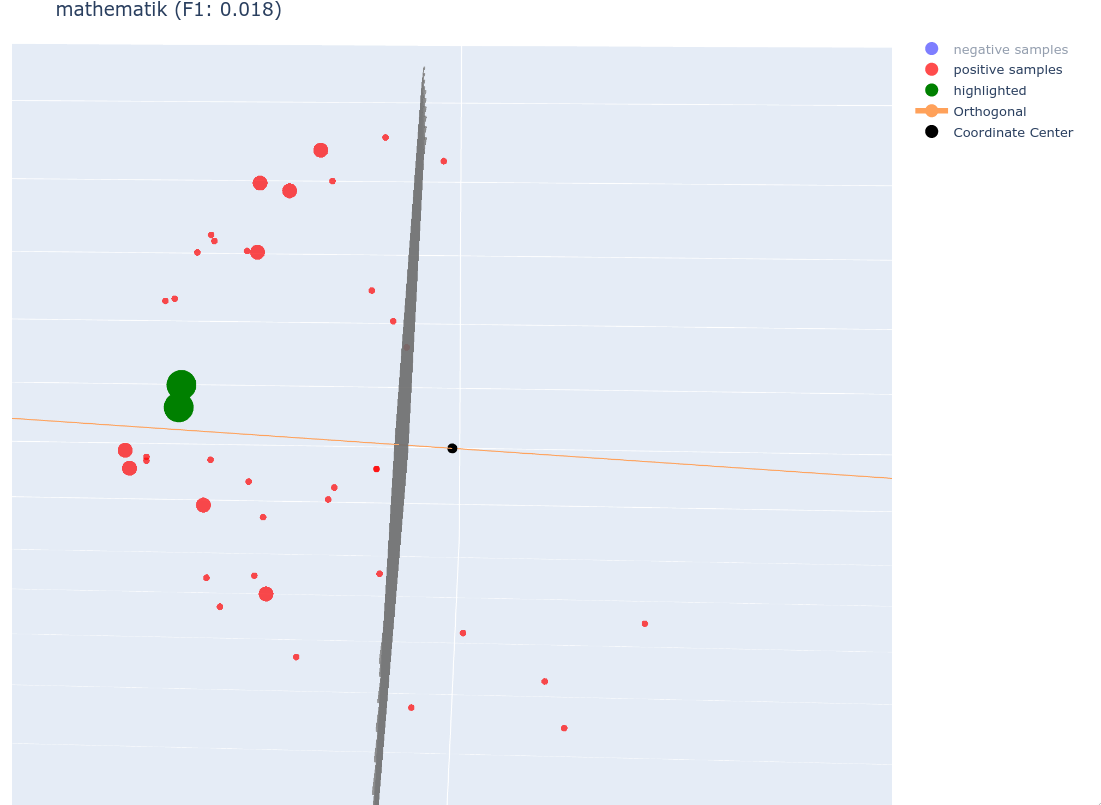
\includegraphics[width=\figwidth]{svm_mathematik_highlight_infoAB.png}
	\caption[3D-Plot with an SVM for the term "Mathematik"]{
		\label{fig:3dplot_mathe_infoab}
		3D-Plot with an SVM for the term "Mathematik", also highlighting the courses "Informatik A" and "Informatik B"
	}
\end{figure}

In figure \ref{fig:3dplot_mathe_infoab} we see a 3D-Embedding for courses, splitting courses which contain the term "mathematics" from those that don't, also hightlighting the terms "Informatik A" and "Informatik B". We see they are close we see the SVM is not to bad, and even though neiher Info A nor Info B contains the word "mathematik", thy are both on the "mathematical side" of courses. Negative samples are hidden for better visibility, and entities that contain the word more-often-than-the 75th (???) percentile have bigger markers.


\begin{itemize}
	\item In 3D ists immer ne Kugel, und ich würde behaupten in höheren Dimensionen ist es nicht extrem viel besser. dadrin ne SVM zu machen bringt echt wenig bis gar nix (Ich hab ja sogar Plots die zeigen dass die Movies viel besser clustern - TODO: die einbringen)
\end{itemize}


\section{Quanitative Results}

Here I'll add the results of the low-depth-decision-trees for Fachbereich, and also compare the results of throwing my code onto their datasets and how my results compare to theirs

Both \cite{Ager2018} and \cite{Alshaikh2020} train shallow decision-trees (depth 1 and depth 3 each), on their feature-based representations (such that the 1 or 3 most distinct interpretable dimensions are used) on a known property of the data (genres for movies, category in some taxonomy for placetypes, fachbereich for mine) - in the assumption that these eg in the movie domain the genre (or rather *terms accurately predicting it*) is among the features.



\chapter{Discussion and Conclusion}
% (was sind die broaden takeaways von meinem Kram)
% * Nochmal nen theoretisches Embedding, Kontextualisieren für Bildungsressourcen
% * ...and conclusion

\section{Future Work}
\begin{itemize}
	\item Evaluation in Stud.IP (which may then even be used for training something like \cite{VISR12}'s algorithm or the fine-tuing step of \cite{Ager2018})
\end{itemize}

\section{Discussion}

In die Conclusion auch die Frage inwieweit das jetzt conceptual spaces sind (sehr viele vereinfachende sachen, like no convex regions but simply dots)
[AGKS18] ist da auch mehr humble als [DESC15] und sagt "The idea of learning semantic spaces with accurate fea- ture directions can be seen as a first step towards methods for learning conceptual space representa- tions from data"


\chapter*{Acknowledgements}
%TODO A place to say thank you to everybody who helped you.


% START Acronym definitions
\newacronym{utc}{UTC}{Universal Time Coordinated}
\newacronym{ml}{ML}{Machine Learning}
\newacronym{svm}{SVM}{Support Vector Machine}
\newacronym{mds}{MDS}{Multi Dimensional Scaling}
\newacronym{ppmi}{PPMI}{Positive Pointwise Mutual Information}
\newacronym{bow}{BoW}{Bag Of Words}
\newacronym{imdb}{IMDB}{Internet Movie Database}
% END Acronym definitions

\glsaddall
\printglossaries %TODO let glossary appear in TOC

%----------------------------------------------------------------------------------------
%	THESIS CONTENT - APPENDICES
%----------------------------------------------------------------------------------------
	
	\appendix % Cue to tell LaTeX that the following "chapters" are Appendices
	
	% Include the appendices of the thesis as separate files from the Appendices folder
	% Uncomment the lines as you write the Appendices
	
	% Appendix A

% \newgeometry{
% 	a4paper,
% 	top=21mm,
% 	bottom=11mm,
% 	inner=24mm,
% 	outer=9mm,
% } %bindingoffset=.5cm

%\newgeometry{
%	a4paper, inner=1.9cm, outer=1.9cm, bindingoffset=1.3cm, top=1.5cm, bottom=1.5cm, 
%} %bindingoffset=.5cm


% \lstset{
% 	numberblanklines=false
% 	,basicstyle=\ttfamily%
% 	,breaklines=true%
% 	,tabsize=1%
% 	,showstringspaces=false%
% 	,numbers=left%
% 	,numbersep=\lstnumbersep%
% 	,numberstyle=\lstnumberstyle%
% 	,framesep=0pt%
% 	,xleftmargin=\lstnumberwidth%
% 	,framexleftmargin=\lsthorizontalpadding%
% 	,xrightmargin=\lsthorizontalpadding%
% 	,framexrightmargin=\lsthorizontalpadding%
% 	,backgroundcolor=\color{verylightgray}%
% 	,postbreak=\ding{229}\space%
% 	,escapeinside={*(}{*)}
% 	\linespread{1.0}
% }


\chapter{Code Use-Cases in Praxis} % Main appendix title

\label{AppendixA} 

\vspace{-0.8cm}

\label{ap:usecase_click}

\label{ap:usecase_snakemake}

\label{ap:usecase_notebook}

\includeMD{pandoc_generated_latex/6_0_usecases}

%\lstinputlisting[language=Python, firstline=29]{codes/dqn.txt}


	% \restoregeometry %TODO do I need separate geometries for the appendices? Bc if I use the package I have to change how I set margins etc!


\printbibliography[heading=bibintoc]

\end{document}
